%!TEX root = ttc16-cra-sigma.tex

\section{Solution Description}
\label{sec:SolutionDescription}

The core of this case study is to transform a RDG model into a high-quality class diagram (\Cf Figure~\ref{fig:Metamodel}).

\begin{figure*}[h!tb]
  \centering
  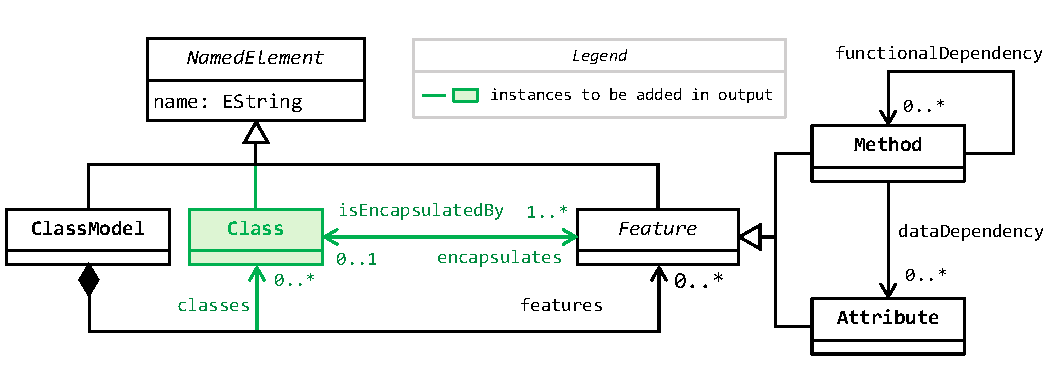
\includegraphics[width=.6\textwidth]{figures/metamodel.pdf}
  \caption{RDG and class model metamodel~\cite{Fleck2016}}
  \label{fig:Metamodel}
\end{figure*}

To consider the quality of a class digram, two common software engineering metrics are used: \emph{coupling} (the number of external dependencies) and \emph{cohesion} (the number of internal dependencies).
The two metrics can be further combined in one, single quality metric called \emph{CRA-Index}, which simply subtracts the coupling from cohesion.
The case study authors provide a set of utility functions that can compute all these metrics from a class digram instance and therefore we do not need to concern ourselves by their precise definitions.

The outline of the solution proposed in this paper is as follows:

\begin{compactenum}
  \item Load the input RDG model from a given XMI file.
  \item Transform the RDG model into MOEA problem instance.
  \item Run the MOEA solver using either NSGA-III or SPEA2 algorithms.
  \item From the possible solutions (which are part of a Pareto optimal front~\Cf below), select the one with the highest CRA-Index.
  \item Transform the selected solution into class digram.
  \item Save the resulting class diagram into XMI file.
\end{compactenum}

\subsection{Transformations}

An optimization problem defines a search space, or the set of possible solutions together with one or more objective functions.
In our case the search space spans are all the valid class diagrams that can represent a given RDG model.
The objectives are:
%
\begin{inparaenum}[(1)]
\item to minimize coupling, and
\item to maximize cohesion.     
\end{inparaenum}

The functions that compute coupling and cohesion ratios from a class diagram are part of the case study description.
What remains is to find the way how to represent the RDG model as a vector of variables that can be used in a evolutionary algorithm to find a solution.
We use a simple integer vector where the index corresponds to the feature index in the input RDG model and the value corresponds to the index of a class in the resulting class diagram.
The range of each vector element is between 0 and the number of features $- 1$ (since we use 0-based indexing).
In the worst case, (\Ie one feature per class), this actually equals to the number of features. 
For example, a vector $\left( 3, 5, \dots \right)$ represents a solution in which first feature belongs to fourth class, second feature to sixth class, and so on and so forth.
Figure~\ref{fig:SolutionOverview} shows a further example of this representation on the example input/output model pair from the case description~\cite{Fleck2016}.

\begin{figure}[h!tb]
  \centering
  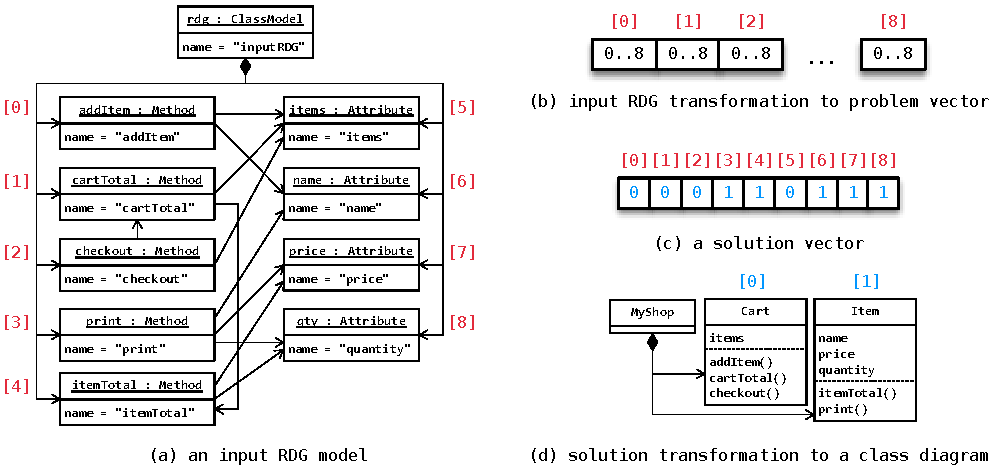
\includegraphics[width=.9\columnwidth]{figures/solution-overview.pdf}
  \caption{Example of the Solution}
  \label{fig:SolutionOverview}
\end{figure}

The advantage of this representation is that it can be easily mapped to MOEA decision variables.
Also, each feature will always be assigned to (encapsulated by) some class.
Therefore, the second validation constraint \emph{all features provided in the input model must be encapsulated by a class}, will be always satisfied without any additional logic.

\enlargethispage{5mm}

Concretely, in the MOEA framework, we have created a \texttt{Problem} class, called \texttt{CRAProblem}.
The integer vector is used to define the decision variables, their types (\Ie integers) and bounds (\Ie $0\dots\text{number of features}-1$).
The number of decision variables corresponds to the number of features in the input RDG model.
The number of objectives is always two, the first one for coupling and the second one for cohesion.
The method instantiating new solution instances looks as follows:
%
\begin{scalacode}
override def newSolution() = {
  val s = new Solution(numVars, numObjs)
  (0 until numVars) foreach (x => s.setVariable(x, newInt(0, numVars - 1)))
  s // return the new instance
}
\end{scalacode}

Next to providing a method to instantiate new instances of solutions for the problem, we need to also define the evaluation of a solution to compute the objectives.
This involves two steps:
%
\begin{inparaenum}[(1)]
  \item transforming the solution into a class diagram
  \item using the provide \texttt{calculateCoupling} and \texttt{calculateCohesion} utility functions to compute the metrics.
\end{inparaenum}
%
In code this is implemented as:
%
\begin{scalacode}
override def evaluate(s: Solution) = {
  val m = solutionToClassModel(initModel, s) // transformation
  s.setObjective(0,calculateCoupling(m))     // minimize coupling
  s.setObjective(1,-calculateCohesion(m))    // maximize cohesion
}
\end{scalacode}
%
The negation of the cohesion ratio is due to the fact that MOEA only works on minimization problems and thus we need to negate the objective value to convert from maximization into minimization.
The following is the code that does the transformation.
This is the main code that uses \SIGMA.
%
\begin{scalacode}
def solutionToClassModel(initModel: ClassModel, s: Solution) = {
  val m = initModel.sCopy // create a new model as a copy of the input one
  val v = EncodingUtils.getInt(solution) // get problem vector (v: Array[Int])
  // create new classes
  val classes = (0 to v.max) map (x => Class(name = s"Class $x"))

  // assignment
  v.zipWithIndex.foreach {
    case (cIdx, fIdx) => m.features(fIdx).isEncapsulatedBy = classes(cIdx)
  }

  // add non-empty classes
  m.classes ++= classes filter (x => !x.getEncapsulates.isEmpty)
  m
}
\end{scalacode}

Finally, we define a new type, \texttt{Solver}, which is a function $RDG \rightarrow ClassDiagram$.
The solver is responsible
%
\begin{inparaenum}[(1)]
  \item to find the Pareto optimal front of all possible solutions (subject to solver configuration), and
  \item to select the solution from that set which has the highest CRA-Index.
\end{inparaenum}
The non-dominated, Pareto optimal front refers to optimal solutions whose corresponding vectors are non-dominated by any other solution vector~\cite{bowman2010solving} and it can be found by MOEA \texttt{Executor}.
For example using the NSGA-III algorithm, we find the non-dominated vector as:
%
\begin{scalacode}
new Executor().withProblemClass(classOf[CRAProblem], initModel)
              .withAlgorithm("NSGAIII")
              .withProperty("populationSize", 64)
              .withMaxEvaluations(10000)
              .run()
\end{scalacode}
%
The individual solutions in this vector are first converted to the class model using the function \texttt{solutionToClassModel}. 
Then we use the given \texttt{calculateCRA} function to find the highest CRA.
To have a better chance to find a good solution, we run each algorithm 10 times (this starts the algorithm from 10 different random seeds).
The properties of each algorithm are defined based on the suggestion by Bowman~\Etal~\cite{bowman2010solving}.

% The code is organized into three classes in \texttt{src/main/scala} folder:
% %
% \begin{compactitem}[---]
%   \item \texttt{CRAProblem} defines the CRA problem in terms of MOEA problem,
%   \item \texttt{Solvers} preconfigures the two used algorithms for the finding the non-dominated solution vector, and finally
%   \item \texttt{Main} that assembles the solution together into an executable application.
% \end{compactitem}